\begin{abstract}
The internet has enabled collaborations at a scale never before possible,
but the best practices for organizing such large collaborations are still not clear.
Wikipedia is a visible and successful example of such a collaboration which might offer
insight into what makes large-scale, decentralized collaborations successful.
We analyze the relationship between the structural properties of WikiProject coeditor networks
and the performance and efficiency of those networks.
We also perform numerical simulations to determine whether social learning on an NK model can
reproduce the behavior observed on Wikipedia.
We find several results seen in numerical and small-scale lab studies:
a performance/efficiency trade-off,
higher performance with less skewed node distributions,
and higher performance with shorter path lengths.
We also see behaviors not previously identified: an association between low degree coeditor networks
and both higher performance and higher efficiency,
suggesting possible benefits to decentralized collaborations made of smaller, more tightly-knit teams.
We also propose a novel consensus-based social learning strategy that is both more efficient and higher
performance than existing strategies, and reproduces some behaviors seen in WikiProjects.
\end{abstract}

\maketitle

\section{Introduction}
\epigraph
{The problem with Wikipedia is that it only works in practice. In theory, it's a total disaster.}
{Gareth Owen \cite{elsharbaty_editing_2016} }

The internet has enabled collaborations at a scale never before possible, a global scale.
Wikipedia is one of the most successful and visible of these collaborations,
and is particularly interesting for its highly decentralized structure with very little top-down control.
It is notoriously difficult to organize even small groups without top-down control
\cite{freeman_tyranny_1972},
and yet Wikipedia, with millions of self-organized editors,
has produced a high-quality encyclopedia \cite{giles_internet_2005,keegan_evolution_2017}.
A better theoretical understanding of projects like Wikipedia is highly desirable as it could
help inform the design of new collaborative projects.
We focus on one aspect of organizing a large-scale decentralized collaboration:
the network structure \cite{newman_structure_2003}.
If Wikipedia is not structured as a top-down hierarchy, how is it structured?
And is that structure related to its success?

We approach these questions by analyzing WikiProjects on the English-language Wikipedia.
WikiProjects are collections of thematically related articles,
each with their own standards, norms, and processes for evaluating and improving articles.
We focus on the coeditor networks of these projects:
which editors have edited at least one article in common?
When measuring the quality of collaborative projects,
there are at least two distinct measures to consider.
The first measure is short-term:
how effective a unit of work is at improving
the collaboration's output,
which we call {\em efficiency}.
The other measure is long-term:
the highest quality typically reached by an output,
which we call {\em performance}.
These two terms are often used interchangably,
but we find it fruitful to distinguish between the two concepts.

Our main findings are:
\begin{itemize}
\item WikiProjects having low-degree coeditor networks tend to have both higher performance and higher efficiency, independent of path lengths;
\item Short path lengths tend to be associated with higher performance, consistent with a conformity-based learning strategy;
\item Structural inequality, as measured by degree skewness, is associated with lower performance,
and lower efficiency at reaching the highest quality levels;
\item Using numerical simulations, we show that the performance and efficiency of some networked learning strategies depends on degree distribution.
\end{itemize}

The rest of the paper is structured as follows.
Section \ref{sec:background} reviews related work and the motivation for the present project,
Section \ref{sec:wp} describes the methodology and results of our empirical analysis of WikiProjects,
Section \ref{sec:sim} describes the methodology and results of our numerical simulations,
Section \ref{sec:discuss} discusses the interpretation and broader impact of our results,
and Section \ref{sec:conclusion} concludes.

\section{Background and Related Work}
\label{sec:background}

The field of social learning studies how
groups of interacting agents
can collaborate to solve complex problems.
In {\em networked social learning},
agents are represented by nodes on a network
and can only interact with their neighbors.
Social learning tasks can be divided into cases where agents have {\em generated signals}
(independently noisy estimates of a true value)
and those where agents have {\em interpreted signals}
(solutions based on different selections of available data)
\cite{hong_interpreted_2009}.
The behavior of individual agents is described by their
{\em social learning strategy}.
For generated signals,
a naive Bayesian approach converges to the truth
when all agents have the same degree,
while the speed of convergence depends on the {\em spectral gap}
between the two largest eigenvalues of the network's adjacency matrix
\cite{degroot_reaching_1974,golub_naive_2010}.
Complex social learning tasks can also be modeled as the problem
of maximizing an objective function with many local maxima,
referred to as a {\em rugged landscape}
\cite{lazer_network_2007,mason_propagation_2008,mason_collaborative_2012,grim_scientific_2013,barkoczi_social_2016}.
Numerical simulations have shown that efficient networks
(those with short paths between nodes)
can result in faster convergence at the cost of a less optimal solution,
due to less time for exploration
\cite{mason_propagation_2008,grim_scientific_2013}.
However, when conformity-based social learning strategies are used,
efficient networks can sometimes find more optimal solutions than
inefficient ones \cite{barkoczi_social_2016}.
The above tradeoff between convergence time, optimality, and learning strategy
motivates the distinction between performance and efficiency in the current study.

Lab-based experiments on networked collaboration
suggest a complex interaction between network topology,
and other factors.
While groups of networked human subjects reliably perform very well on
difficult graph-coloring tasks, the best performing network architectures
(e.g., fully-connected vs. small-world) vary
from task to task \cite{kearns_experiments_2012}.
The same studies found that while human subjects tend to perform very well on
a number of networks, they perform worst on collaboratively self-organized
networks, highlighting the importance of intentionality
in constructing communication channels for collective decision-making.
Similarly, some network topologies are able to reach faster decisions in the
presence of more information, while others show the opposite effect
\cite{kearns_experimental_2006}.
Based on lab experiments, Fowler and Christakis \cite{fowler_cooperative_2010}
suggest that individual decisions towards altruism are conditional on their
neighbor's behavior and ``contagious'' up to three degrees away.
Later experiments by Suri and Watts \cite{suri_cooperation_2011} confirmed the
existence of conditional altruism,
but concluded that altruistic
behavior only influences first-degree neighbors.
While theories of networked social learning have been tested in small-scale lab experiments,
there is a need to study real-world, large-scale collaborations,
as we do in the present paper.

In addition to learning, decision-making is a crucial component of collaboration.
The Condorcet jury theorem and its extensions \cite{list_epistemic_2001}
describe how individuals can use majority voting to improve their
decision-making ability.
The process of decision-making is sometimes divided into
``talking'' and ``voting'' stages.
% Not yet published
%While hierarchical representative democracy sometimes improves the outcome
%of ``talk,'' it weakens the result of the Condoret jury theorem for voting
%\cite{}.
Robert Michels proposed the ``iron law of oligarchy,''
\cite{michels_political_1999} which states that
the earlier members of a group will, over time, gain disproportionate
decision-making power and act increasingly out of self-interest rather than
the good of the group.
Shaw and Hill found that behavior in online wiki communities is consistent
with the iron law \cite{shaw_laboratories_2014}.
A number of studies, summarized in \cite{gentry_consensus_1982},
have examined consensus-based decision-making procedures, used extensively by
the Quakers and later by activist communities.
The hallmark of consensus is the equal and active participation by all members
of a group.
Key findings include the trade-off between speed and quality of decisions,
the importance of expressing conflict early in the process,
and the willingness to recognize when one's own views are counter to the
existing consensus.
De Tar created InterTwinkles \cite{detar_intertwinkles:_2013},
an online suite of tools to facilitate consensus decision-making
in small cooperatives.
Consensus decision making is notoriously difficult to apply in large groups.
Wikipedia is one of the largest collaborations to use consensus-based
decision-making,
making it an excellent place to study the role of network structure in
large-scale collaboration.

Research on digital communities has also examined the role of factors
such as diversity and inequality
in collaborative work and decision-making.
Using a simulation model, Hong and Page \cite{hong_groups_2004} found that
diverse groups can outperform groups composed of the best individual
problem-solvers.
In sociology, much research has been done examining the relationship between
network structure and social capital.
Powerful individuals are often ``brokers''
who act as exclusive intermediaries between disconnected portions of the
social network \mbox{\cite{silverman_patronage_1965}}.
Similarly, successful innovation in organizations often occurs in ``structural
holes'' between groups \mbox{\cite{granovetter_strength_1973}}.
There is some evidence that groups with high structural inequality,
as evidenced by highly-skewed degree distributions,
perform worse on collaborative tasks \mbox{\cite{kearns_experiments_2012}}.
In the present project, we use co-editor network degree skewness to
examine the relationships between structural inequality,
project performance, and project efficiency.

Several studies have examined the role of community in the specific context
of Wikipedia.
Robert and Romero found that
larger group sizes yield higher article ratings
(as determined by editor peer-review)
when the groups are diverse and experienced
\cite{robert_crowd_2015}.
Also on Wikipedia,
Kittur and Kraut found that different types of coordination have a complex
effect on the quality of Wikipedia articles \cite{kittur_harnessing_2008}.
Both explicit and implicit coordination result in higher quality articles,
with explicit coordination being especially central in the early life of an
article.
Looking specifically at Wikipedia policies determined by editor consenus,
Keegan and Fiesler found a trend
from flexibile rule-making towards less flexible maintenance and deliberation
\cite{keegan_evolution_2017}.

Across the broad range of work discussed above,
a few key themes emerge.
The efficiency and performance of collaborations are important considerations
and vary depending on both network structure and type of task
\cite{kearns_experiments_2012}.
While generated signal models of social learning predict no relationship between the two
\cite{golub_naive_2010},
contagion-style innovation models predict a trade-off
\cite{mason_collaborative_2012,barkoczi_social_2016}.
Such a trade-off has been observed in simulations and lab experiments on
collaboration
\cite{kearns_experiments_2012,grim_scientific_2013}.

In this project, I will investigate several gaps in the existing literature.
In much of the existing literature,
degree distribution correlates to performance.
But aside from the naive Bayes case in social learning, it is unknown whether
the correlation is explained best by degree or by another structural property
correlated with degree.
The characteristic path length and min-cut studied here are candidates for such
degree-correlated factors.
While existing work has focused on families of artificial networks,
this project examines a large number of naturally-occurring networks.
Unlike artificial networks, the structural properties of these naturally-occurring
networks can vary independently, making it easier to isolate individual
network properties that correlate with outcome variables.
This project will also examine Wikipedia for evidence that structural
inequality (in the form of skewed degree distributions)
has relationship with performance,
as has been observed in lab experiments
\cite{kearns_experiments_2012}.

\section{WikiProjects}
\label{sec:wp}

Many articles on Wikipedia belong to one or more WikiProject.
WikiProjects are groups of thematically-related articles
(e.g., articles related to Philosophy).
Information about the an article's associated WikiProjects
can be viewed on that
article's talk page (Figure \ref{fig:knitting}).
Each WikiProject has its own page and talk page.
These pages contain information about community norms within the project
as well as discussions about individual articles.
WikiProjects are thus distinct communities, with distinct norms and processes.
These communities are the fundamental units of analysis in the present paper.

One of the main roles of a WikiProject is to evaluate the quality of its articles.
Quality assessments are made through consensus-based deliberation on the WikiProject
talk page.
Within a WikiProject,
assessments are typically made using the following {\em assessment classes}
(in order of increasing quality):
Stub, Start, C, B, A.
Different WikiProjects can assign different quality assessments to the same
article.
Differences between quality assessments could reflect different quality standards,
different grading systems, different responsiveness to changes in an article, etc.

In addition to the above assessment classes, articles on Wikipedia can be tagged as
"good article" (GA) or "featured article" (FA) quality.
FA and GA determinations are made using a Wikipedia-wide consensus,
in parallel to any WikiProject-based evaluations.
FA articles are ``the best articles Wikipedia has to offer''
\cite{}.
GA articles meet ``a core set of editorial standards`` but are ``not featured article quality''
\cite{}.
When an article is assigned GA or FA status,
WikiProject quality assessments are often updated to reflect that status.
For example, the article {\em Mewtwo} was assessed as GA status on October 5,
2009 and shortly afterwards
its quality assessment was changed from B to GA within both
{\em WikiProject Pok\'emon} and
{\em WikiProject Video Games}.
This example also illustrates a quirk of Wikipedia norms:
very often, articles pass to GA or FA directly from B, skipping A.
The majority of WikiProjects rarely use the A class quality assessment.

\begin{figure}
\begin{center}
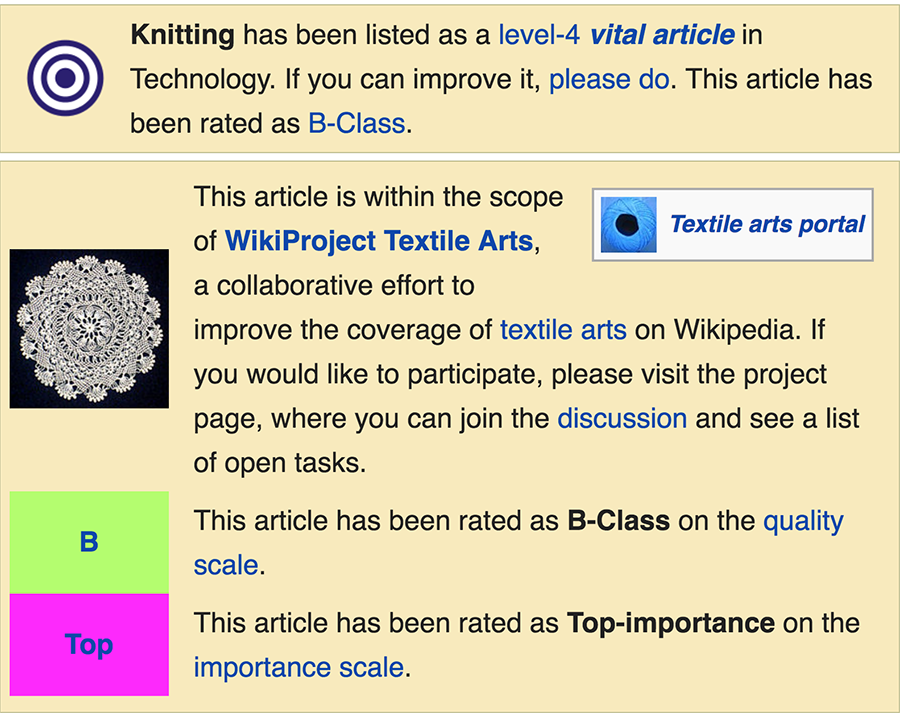
\includegraphics[width=3in]{fig-knitting.png}
\caption{
Templates appearing at the top of the English-language Wikipedia talk page
for {\em Knitting}.
The article belongs to both {\em WikiProject Technology} and
{\em WikiProject Textile Arts}.
Both WikiProjects have assessed the article as B-class quality.
The article has also been nominated for both good article (GA) and
featured article (FA) status,
but after a consensus-based deliberation open to all Wikipedia editors,
was not assigned GA or FA status.
\label{fig:knitting}
}
\end{center}
\end{figure}

\subsection{Data}

Our analysis combines multiple data sets from the English-language Wikipedia.
For information about edit history, we used a publicly-available data set containing
metadata about all edits from July 12, 2006 to December 2, 2015.
To get the rating history of each article,
we wrote a script to scrape the daily logs produced by WP 1.0 Bot for
all unique WikiProjects (2279)
between May 4, 2006 and December 2, 2015.
Finally, we used a publicly-available log of page events (including rename events)
to reconstruct the unique identifier for each article title mentioned in the rating history logs.

\subsection{Efficiency and Performance}

When individuals collaborate to solve a problem,
there are many ways to gauge their success.
Two possibilities are
1. how quickly they find a solution, and
2. how good their solution is.
Evidence from numerical simulations
\cite{lazer_network_2007,mason_propagation_2008,mason_collaborative_2012,grim_scientific_2013,barkoczi_social_2016},
lab studies \cite{kearns_experiments_2012},
and field observations \cite{gentry_consensus_1982}
all suggest a trade-off between performance and efficiency.
While common, this trade-off is not absolute,
suggesting it is sometimes possible to simultaneously increase
performance and efficiency.
The identification of factors associated with both higher efficiency
and higher performance has obvious practical importance.
In this paper, we focus specifically on how network structure
relates to efficiency and performance within WikiProjects.

For a WikiProject, efficiency quantifies how much participants can raise the
assessed quality of an article for a fixed amount of work.
We measure work by the number of revisions made.
Quality assessments are made through consensus of the project participants themselves,
so different projects can have different standards and practices for assessing article quality.
So the efficiency is not a measure of how quickly some objective measure of quality improves,
but rather of how quickly the project participants can reach consensus on the improvements that
need to be made and make those improvements.
Because our definition relies on assessment transitions,
we must define efficiency variables for
each of the project-level quality assessments: A, B, and C.
For a particular grade $G$,
we desire our definition of efficiency to meet the following conditions:
\begin{itemize}
\item{Strictly increasing in the number of articles reaching grade $G$ (with revision count fixed);}
\item{Strictly decreasing in the number of revisions (with transition count fixed);}
\item{Independent of WikiProject size: not affected by adding an article if that article's transition/revision ratio is equal to the efficiency.}
\end{itemize}

We now define an efficiency measure which meets the above criteria.
Let $T(W,G)$ be the set of article assessment transitions from below grade $G$
to grade $G$ or higher in project $W$.
Let $N(W,G)$ be the number of articles in project $W$ which ever transition
from below grade $G$ to grade $G$ (or higher).
Let $r(t)$ be the number of article revisions since its previous grade transition,
and let $g(t)$ be the number of grade levels crossed by transition $t$.
We quantify the efficiency $E(W,G)$ as the inverse of the mean number of revisions
per transition:
\beq
E(W,G)
&=&
\left[
\frac{1}{
N(W,G)
}
\sum_{t \in T(W,G)} \frac{r(t)}{g(t)}
\right]^{-1},
\eeq
Where the $g(t)$ term is present because a assessments sometimes raise article quality by several
grades, in which case we divide the revisions evenly between all grade levels achieved.

For performance, we wish to quantify how good articles tend to be when they reach a stable state.
Measuring performance is difficult for several reasons:
there is no objective measure of article quality available,
and articles are always changing, making it difficult to know which articles should be considered
complete or stable.
We use an extremely simple performance measure that gives surprisingly consistent results.
In addition to per-project quality assessment, articles can be given ``featured article'' or
``good article'' status.
The criteria for these statuses are consistent across all of Wikipedia,
and any editor can participate in the discussion and decision to award good or featured
status.
In other words, the good and featured statuses are more objective than per-project assessments.

Our performance measure $P(W)$ is defined simply as
the percentage of articles in project $W$ which have reached
good or featured status:
\beq
P(W) &=& \frac{f(W) + g(W)}{n(W)},
\eeq
where $f(W)$ and $g(W)$ are the numbered of featured and good articles respectively,
and $n(W)$ is the total number of articles.

\subsection{Coeditor Networks}

We would like to determine how the social network structure of
Wikipedia--the pattern of who interacts with whom--relates to
efficiency and performance.
There are several types of interactions we could focus on,
including:
coediting, user talk messages, and talk page replies.
We choose to focus on coediting: when two editors have made changes to the
same article or talk page.
While editors can communicate directly through user talk messages,
the number of such messages is small compared to the number of edits to article
and talk pages.
We also could have considered direct replies between editors on article talk
pages, but these replies are typically seen (and intended to be seen)
by everyone reading the talk page,
and are part of larger conversations.
When an editor views a page,
they are potentially viewing content from and interactions
between all editors who came before them,
motivating our choice to focus on the social network structure of
coeditors.

The {\em coeditor network} of a WikiProject consists of nodes representing editors,
and edges connecting any editors who have edited the same article.
The edges are directed, with the direction representing the direction of
{\em plausible information flow};
an edge from Alice to Bob exists if Alice edited an article and then Bob edited the same article at
a later time.
Edges can exist in both directions e.g.,
if an article was edited first by Alice, then by Bob, and again by Alice.
We make the simplifying assumption of unit weight for all edges.
We focus on three structural properties:
degree, characteristic path length, and min-cut.
Degree and characteristic path length have been shown to correlate with
performance and efficiency in some social learning settings
\cite{golub_naive_2010,mason_propagation_2008,grim_scientific_2013},
while min-cut can be interpreted as a measure of decentralization,
common feature of peer-produced communities such as Wikipedia
\cite{benkler_wealth_2006}.

The degree distribution is the simplest network property we analyze.
The in-degree (out-degree) of a node is the number of edges to (from) that node.
Taking the average of either in-degree or out-degree gives the same value:
the {\em mean degree} of the network.
In our context, the mean degree represents how many others a given editor has collaborated with.
We also consider the {\em skewness} of the in-degree and out-degree distributions.
A large positive degree skewness value for a WikiProject coeditor network
implies that a small number of editors have a very large number of collaborators,
while a small positive value implies that the editors having the most collaborators
don't have many more than a typical editor.

We also calculate the characteristic path length for each WikiProject coeditor network.
The {\em distance} from node $s$ to node $t$ is the distance of the shortest path
from $s$ to $t$.
The {\em characteristic path length} (or just {\em path length} for brevity)
is the mean distance between all editor pairs,
excluding unconnected pairs.
To account for unconnected pairs, we also measure the {\em connected fraction}
of all possible edge pairs.
The path length represents how quickly information can move through the network.
Networks with longer paths require more interactions for information to propagate through
the network,
which has been shown to reduce efficiency in some settings
\cite{mason_propagation_2008,barkoczi_social_2016}.

Our final network measure quantifies the connectivity of a project's coeditor network using
min-cut size.
The minimum $st$-cut between nodes $s$ and $t$ is the set of edges that must be removed in order that
no path exists from $s$ to $t$.
The minimum cut (min-cut) of a graph is the smallest minimum $st$-cut over all node pairs $st$. 
The size of the graph min-cut quantifies the connectivity of a graph,
but only incorporates information about edges lying on paths crossing the min-cut.
Instead, we use the mean size of all minimum $st$-cuts, which we refer to as the
{\em mean min-cut}.
This measure quantifies the number of redundant paths information can take through the network.
Networks with higher redundancy are more resilient to errors on one path \cite{albert_error_2000}
and allow innovations to propagate through complex contagion,
in which innovations are only adopted after multiple exposures through different sources
\cite{centola_complex_2007}.

The mean path and min-cut network measures are computationally intensive,
requiring distance and minimum $st$-cut calculations for each all node pairs.
For larger projects, these calculations are impractical.
When coeditor networks were large, we employed sampling to determine mean path length and mean
min-cut.
For mean path length, source nodes were sampled, and path length was calculated to all destination nodes
from each of these.
For min-cut, node pairs were sampled.
In both cases, stratification was used to ensure the same number of nodes were were sampled from each of
12 node degree quantiles.
We estimated the error due to sampling by determining true values for a medium-sized project,
and calculating error as a function of sample-size.
Sample sizes were chosen such that relative error was below 10\%.
Even with sampling, however, it was impractical to calculate these properties for the largest projects,
so we exclude the 183 largest projects from the analysis.
To control for bias in project size, we include several size-related variables in our models.

\subsection{Empirical Results}

We find that both efficiency and performance are highly right-skewed,
with a small number of projects having values much higher than the average.
After log-transforming the values, both the efficiency and the performance have
a unimodal distribution with low skew (see Figure \ref{fig:eff-perf-hist}).

We also find that mean min-cut is highly correlated with degree ($r=0.980$, $p<0.001$),
so we exclude min-cut from regression models to prevent collinearity (see Figure \ref{fig:degree-mincut}).
The high correlation between mean degree and min-cut implies that in most cases
the minimum $st$-cut is simply the either set of edges from $s$ or the set of edges to $t$.
The rarity of non-trivial min-cuts suggests that WikiProject coeditor networks have very few central
bottlenecks and are thus highly decentralized.

\begin{figure}
\centering
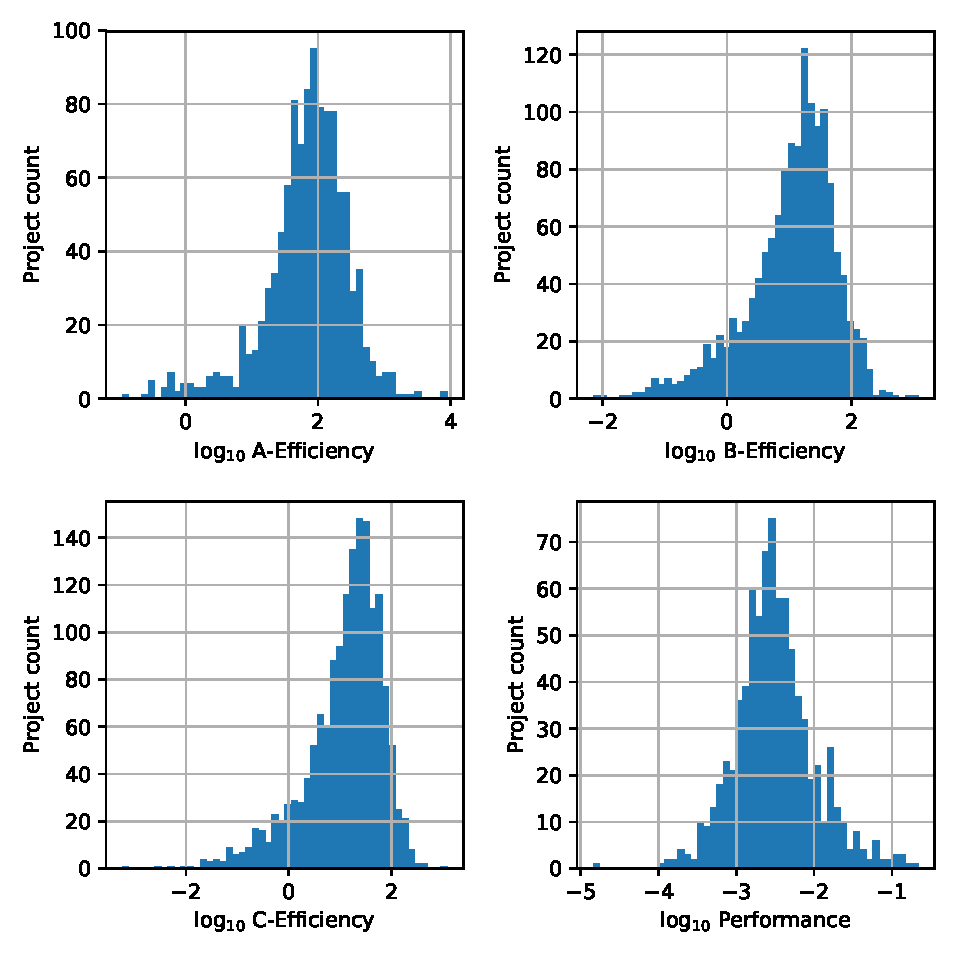
\includegraphics[width=3in,height=3in]{fig-eff-perf-hist.pdf}
\caption{
Histograms of WikiProject efficiency and performance.
Both measures are highly right-skewed, but form unimodal distributions
with low skewness after log transformation.
\label{fig:eff-perf-hist}
}
\end{figure}

\begin{figure}
\centering
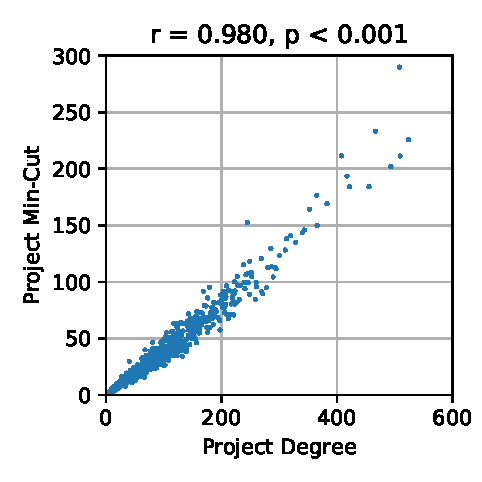
\includegraphics[width=2.33in,height=2.33in]{fig-degree-mincut.pdf}
\caption{
Min-cut of WikiProject coeditor networks vs. their mean degree.
\label{fig:degree-mincut}
}
\end{figure}

\begin{table*}[!ht]
\small
\caption{Standardized coefficients for OLS models.
\label{tab:model}
}
\bigskip
\begin{tabular}{lllllllll}
\hline
                               & Perf$_1^\dagger$ & Perf$_2^\dagger$ & A-Eff$_1^\dagger$ & A-Eff$_2^\dagger$ & B-Eff$_1^\dagger$ & B-Eff$_2^\dagger$ & C-Eff$_1^\dagger$ & C-Eff$_2^\dagger$ \\
\hline
Mean degree$^\dagger$          &  -0.84$^{***}$  &  -0.78$^{***}$
                               &  -0.61$^{**}$   &  -0.84$^{***}$
                               &  -0.50$^{***}$  &  -0.61$^{***}$
                               &  -0.34$^{**}$   &  -0.31$^{*}$ \\
In-degree skewness$^\dagger$   &  -0.58$^{***}$  & \+ ---      
                               &  -0.43$^{**}$   & \+ ---      
                               &  -0.19          & \+ ---      
                               &  -0.1           & \+ ---      \\
Out-degree skewness$^\dagger$  &  \+ ---         &  -0.48$^{***}$  
                               &  \+ ---         &  -0.57$^{***}$
                               &  \+ ---         &  -0.26$^{*}$
                               &  \+ ---         &  -0.066 \\
Mean path$^\dagger$            &  -0.357$^{***}$ &  -0.356$^{***}$ 
                               &  -0.026         &  -0.096
                               &  -0.020         &  -0.045
                               &  -0.092$^{**}$  &  -0.086 \\
C-eff$^\dagger$                &  -0.083$^{**}$  & -0.085$^{**}$  
                               &  \+ ---         & \+ ---      
                               &  \+ ---         & \+ ---      
                               &  \+ ---         & \+ --- \\
Connectivity                   & \+0.018         & \+0.016        
                               & \+0.081         & \+0.088
                               & \+0.126$^{***}$ & \+0.142$^{***}$
                               & \+0.080$^{**}$  & \+0.081$^{**}$ \\
Mean editors/article$^\dagger$ & \+0.37$^{***}$  & \+0.40$^{***}$ 
                               & \+0.22          & \+0.27
                               & \+0.20          & \+0.22$^{*}$
                               & \+0.076         & \+0.075 \\
Article count$^\dagger$        &  -0.32          & -0.27          
                               & \+0.63${^*}$    & \+0.70${^*}$ 
                               & \+0.76$^{**}$   & \+0.78$^{**}$
                               & \+0.67$^{***}$  & \+0.67$^{***}$ \\
Editor count$^\dagger$         & \+0.68$^{*}$    & \+0.48         
                               & \+0.74$^{*}$    & \+0.97$^{**}$
                               & \+0.60$^{*}$    & \+0.72$^{**}$
                               & \+0.52$^{*}$    & \+0.46$^{*}$ \\
Revision count$^\dagger$       & \+0.37          & \+0.39         
                               &  -0.84$^{**}$   & -0.88$^{**}$
                               &  -1.05$^{***}$  & -1.05$^{***}$
                               &  -1.00$^{***}$  & -1.00$^{***}$ \\
First assessment               & \+0.028         & \+0.058        
                               & \+0.086$^{*}$   & \+0.101$^{**}$
                               & \+0.309$^{***}$ & \+0.321$^{***}$
                               & \+0.456$^{***}$ & \+0.460$^{***}$ \\
Mean article age               &  -0.040         & -0.029         
                               &  -0.049         & -0.037
                               &  -0.019         & -0.014
                               &  -0.046$^{*}$   & -0.045$^{*}$ \\
\hline
DoF                            & 1278            & 1278          
                               & 1048            & 1048
                               & 1371            & 1371
                               & 1540            & 1540 \\
R$^2_{adj}$                    & 0.37            & 0.37          
                               & 0.15            & 0.16
                               & 0.30            & 0.30
                               & 0.43            & 0.43 \\
\hline
\end{tabular}
\begin{tablenotes}
\item $\dagger$ Log-transformed. * $p < 0.05$. ** $p < 0.01$. *** $p < 0.001$.
\end{tablenotes}
\end{table*}

To study the relationship between network structure, efficiency, and performance,
we model the performance and efficiency of WikiProjects using ordinary least-squares linear regression.
Each WikiProject is taken as a single observation.
The models include each project's coeditor network properties as independent variables.
We also include several project-level variables to control for confounding factors,
described below.
\begin{description}
\item[C-efficiency] Quantifies how quickly a WikiProject improves low-quality articles.
\item[Connected fraction] Fraction of coeditor pairs connected by a path.
\item[Mean editors/article] Mean number of editors collaborating on each article in a WikiProject.
\item[Article count] Total number of articles in the WikiProject.
\item[Editor count] Total number of editors working on articles within a WikiProject.
\item[Revision count] Total number of revisions to articles in a WikiProject.
\item[First assessment] Timesamp of first assessment; a measure of how long a WikiProject has been active.
\item[Mean article age] Mean age of articles within a WikiProject.
\item[Mean similarity] Mean Jaccard similarity (by article) with other WikiProjects; a measure of topical complexity.
\end{description}

Our models are summarized in Table \ref{tab:model}.
Min-cut is excluded from all models to avoid collinearity,
as it is highly correlated with degree.
In-degree and out-degree skewness were also highly correlated,
so we only include out-degree skewness in the models.
Some variables are log-transformed.
To test the robustness of our results,
we also computed models using cube root instead of logarithmic transformations,
as well as using only top-importance and high-importance articles.
These robustness check yielded qualitatively similar results for all variables,
except for degree-skewness, which had an inconsistent sign across models.

We see that B-efficiency and C-efficiency have very similar models, but that A-efficiency behaves
differently in its dependence on degree skewness and connectivity.
The different behavior of A-efficiency is likely explained by the observation that the A-Class quality is
infrequently used in practice, meaning that the quality level is usually achieved when an article is rated
as a good or featured article, which involves a different consensus process than lower ratings.

The negative dependence of performance on C-efficiency suggests there is generally a trade-off between
performance and efficiency.
However, low degree is correlated with both higher efficiency and higher performance,
suggesting that it is sometimes possible to improve both simultaneously.
Much of the existing numerical work on networked social learning focuses on path length rather than degree,
so we explore this result further using simulations in the next section.

For path length, we find that longer lengths correspond to lower performance, contrary to the conjecture
that longer path lengths allow more exploration \cite{mason_propagation_2008}
but consistent with a conformity-based social learning strategy \cite{barkoczi_social_2016}.

We also observe that high degree skewness is correlated with lower performance and lower A-efficiency,
suggesting that articles in projects with decentralized coeditor networks reach featured or good status
more efficiently, and reach higher quality ratings in general.

\section{Agent-Based Model}
\label{sec:sim}

In addition to our empirical study,
we use a simple agent-based model of collaboration to better understand
the relationship between node degree, efficiency, and performance.
Numerical models allow us to determine the effect of changing a single
variable (e.g., network strucutre, learning strategy),
which is impractical in the empirical setting.
It is important to note that the goal of our model is not to create an
accurate simulation of Wikipedia or any other specific platform.
Rather, our goal is to simulate collaboration in the abstract so that we can
examine the results of altering various assumptions and parameters.

Past work in the field of social learning typically models collaboration
as an optimization problem:
finding a state of the world which maximizes some objective function
\cite{lazer_network_2007,mason_propagation_2008,mason_collaborative_2012,barkoczi_social_2016}.
Wikipedia itself can be regarded as an optimization problem.
On Wikipedia, editors are generally seeking to improve the quality of articles
and have some personal preference over possible states of an article.
When editors do not agree on the optimal state of an article,
the conflict is resolved through a consensus-based deliberation.
This consensus process can be regarded as a {\em social choice function}
\cite{arrow_social_2012,brandt_computational_2012}
which maps individual preferences to community preferences.
Wikipedia can thus be thought of as a group of editors with individual preferences
for article states,
collaborating to optimize articles according to community preferences.

To simulate collaboration, we need a model problem for collaborators to solve.
Following existing literature on social learning,
we use the NK model \cite{kauffman_towards_1987}
to create NP-hard, nonlinear optimization problems.
The NK model produces an objective function with a
{\em rugged landscape}, i.e., many local optima.
The ruggedness of the model can be tuned through the parameters $N$ and $K$.
Formally, the NK model produces a function $F$ mapping a binary string $S$ of length
$N$ to a real value in $[0,1]$.
The model consists of $N$ {\em loci}, with locus $i$ having a binary state $S_i$
and a value $f_i(S)$ dependent on its own state
and on the state of $K$ random other loci.
The functions $f_i(S)$ are created by selecting a random value in $[0,1]$ for
each possible state of locus $i$ and its $K$ neighbors.
The value of the model $F(S)$ is the mean of all locus values $f_i(S)$.
In our models,
agents thus seek to find a bit string $S$ that achieves the largest $F(S)$.

In a typical social learning model,
a set of agents each maintain an estimate of the optimal state
and iteratively update that estimate based on information available from other agents,
according to some {\em learning strategy}.
In networked social learning,
agents are associated with the nodes of a network and share information
only with their neighbors.
We define efficiency and performance in terms of the solution values for each time step
(averaged over many trials).
We define the performance to be the mean solution value after the process has converged,
while the efficiency is the reciprocal of the number of steps required to converge.
We measure the time to convergence as the number of steps required to reach 99\% of the maximum
mean solution value.

Without additional constraints,
the above model is missing
several key properties of real-world collaborations.
In designing our agent-based model, we paid attention to the
following properties, motivated by real-world collaborations.
\begin{description}
\item[Limited concern] Agents are concerned only with a subset of the entire
state when making decisions and determining preferences.
\item[Concern-based network] Agents interact with other agents who share a
common concern over some subset of the state.
\item[Unknown objective] Agents can rank states in order of preference,
but do not have access to the objective function.
\item[Single source of truth] At any given time, the system is in a single state
and agent preferences are based on local modifications to that state.
\end{description}

\subsection{Concern-Based Networks}

On Wikipedia, editors interact by editing articles and talk pages.
Thus, the editors who interact with each other are exactly those who care about the same content.
Rather than using arbitrary networks,
we devise a network structure inspired by the above observation.
We do so by associating agents with particular loci in the NK model.
We also wish to study the effect of varying network degree,
which we achieve through a rewiring process described below.

Our concern-based networks are generated directly from the structure of the NK model.
The value of each NK locus depends on its own state and the state of $K$ other loci.
For each locus, we define an agent and assign these $K+1$ loci as its concern.
Next, an agent-agent co-affiliation network is created by connecting two agents if they share at least
one locus in their concerns.
This process is analogous to our construction of WikiProject coeditor networks.

To create a tunable degree, we duplicate each agent and its concern,
then randomly rewire a fraction of agent concerns before creating the agent-agent network.
With no rewiring, the duplication process creates a high overlap between agent concerns.
This overlap results in redundant links to a small number of agents,
rather than unique links to a large number of agents,
and therefore to an agent-agent network with small average degree.
By randomly rewiring the agent concerns, the redundancy is reduced
and the average degree of the agent-agent network is increased.

\subsection{Networked Learning Strategies}

Learning strategies determine how agents update their preferences based on
available information.
Agents can engage in individual learning \cite{barkoczi_social_2016}
by applying a hill-climbing algorithm to their current solution.
In each iteration, one bit of the NK solution string is flipped to maximize the solution value.
If no change improves the value, the original solution is kept
The above strategy relies only on rankings of states,
satisfying the unknown objective assumption.
However, it does rely on information about the entire state,
violating the limited concern assumption.
In order to satisfy this assumption,
we also define a local variant
in which only a subset of bits in the NK solution string are considered.
This variant reflects a more realistic style of collaboration,
in which individual agents focus on sub-problems.

In social learning,
agents can also incorporate information from
other agents they are connected to by a network edge.
While individual learning always converges to the local maximum relative to the starting point,
social learning strategies allow agents to ``jump'' to drastically different solutions with higher local maxima.
In our model, we use both the conformity and best-neighbor strategies from \cite{barkoczi_social_2016}.
In the {\em best-neighbor} strategy, each agent compares its solution to a sample of its
neighbors, and chooses the solution with the highest value.
In order to compare solutions between neighbors,
the exact value of the objective function must be known for each solution,
so this strategy does not satisfy the unknown objective assumption
or the limited concern assumption.
In the {\em conformity} strategy, agents simply choose the most common solution among their neighbors
(ties are broken uniformly at random).
This strategy does not rely on solution value at all, so clearly satisfies the
unknown objective assumption,
but it fails to satisfy the limited concern assumption because it updates all
bits of the NK solution.
In both cases, a single iteration of individual learning is performed after each social learning
iteration.
Because each agent maintains a separate estimate of the solution,
neither of these strategies satisfies the single source of truth assumption.

\subsection{Local Majority Strategy}

In order to satisfy the single source of truth assumption,
we introduce a new strategy, which we call the local majority strategy.
In {\em local majority}, agents begin with exactly the same starting state,
and apply individual learning to their concern to generate
possible improvements to the solution.
Next, a new solution is constructed by considering each locus of the NK solution
individually.
Every agent concerned with a bit votes for its state based on their preferred
new solution and the majority state is chosen.
The result of this process is that all agents agree on a single improved state,
which forms the basis for the next iteration.
This strategy more realistically reflects collaborations like Wikipedia:
at any given time, a Wikipedia article has a single state, determined by consensus,
but editors may have differing opinions on how to improve that article.

\subsection{Simulation results}

We simulated 100 trials for rewiring values of 0.0, 0.167, 0.333, 0.5, 0.667, 0.833, and 1.0.
For each trial we generated an NK model with N=250 and K=7 and ran each social learning strategy
for 300 iterations,
as well as a network based on that NK model and rewired.
We confirmed that all trials converged to their maximum value before reaching the last iteration.
Some statistics on the network properties of the networks are summarized in Table \ref{tab:stats}.
We see that the coefficient of variation of degree is approximately 10\%,
while only 1\% for mean path length, confirming that the rewiring process has a stronger influence
on degree than on path length.

\begin{table}
\small
\centering
\caption{
Simulated network statistics.
\label{tab:stats}
}
\bigskip
\begin{tabular}{lcc}
\hline
Property          & Mean  & Std. Dev. \\
\hline
Mean Degree       & 132.3 & 9.2 \\
Mean Path length  & 1.735 & 0.019 \\
\hline
\end{tabular}
\end{table}

\begin{figure}
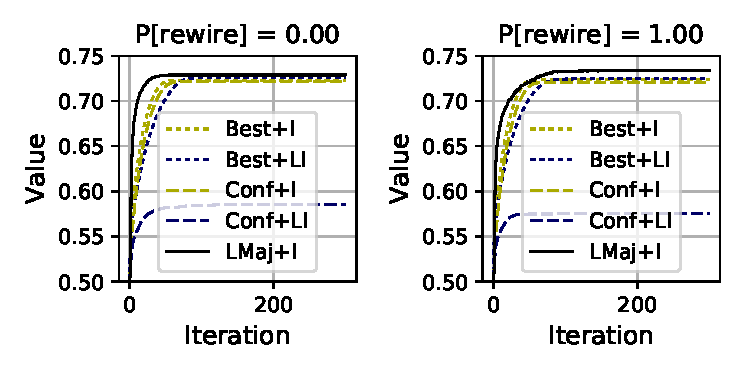
\includegraphics[width=3in,height=1.5in]{fig-val-iter.pdf}
\caption{
Mean agent solution value over time, averaged over 100 trials.
The left and right figures show results for agent networks with the probability of
rewiring set to 0 and 1, respectively.
In both, local strategies are less efficient and more performant than non-local.
The consensus strategy is both more efficient and more performant than others,
with its performance increasing with higher rewiring.
\label{fig:val-iter}
}
\end{figure}

\begin{table}
\small
\caption{
Efficiency regression coefficients.
\label{tab:sim-eff}
}
\centering
\bigskip
\begin{tabular}{llc}
\hline
Strategy & Std. Coeff. \\
\hline
Best-neighbor       & -0.064 \\
Conformity          & -0.080 \\
Local best-neighbor & -0.086 \\
Local conformity    & \+0.049 \\
Consensus           & -0.0325$^{***}$ \\
\hline
\end{tabular}
\begin{tablenotes}
\item \centering * $p < 0.05$. ** $p < 0.01$. *** $p < 0.001$.
\end{tablenotes}
\end{table}

\begin{table}
\small
\caption{
Performance regression coefficients.
\label{tab:sim-perf}
}
\centering
\bigskip
\begin{tabular}{llc}
\hline
Strategy & Std. Coeff. \\
\hline
Best-neighbor       & \+0.084 \\
Conformity          & \+0.130 \\
Local best-neighbor & -0.080 \\
Local conformity    & -0.020 \\
Consensus           & \+2.38$\times{10^{-4\;**}}$ \\
\hline
\end{tabular}
\begin{tablenotes}
\item \centering * $p < 0.05$. ** $p < 0.01$. *** $p < 0.001$.
\end{tablenotes}
\end{table}

\begin{figure*}
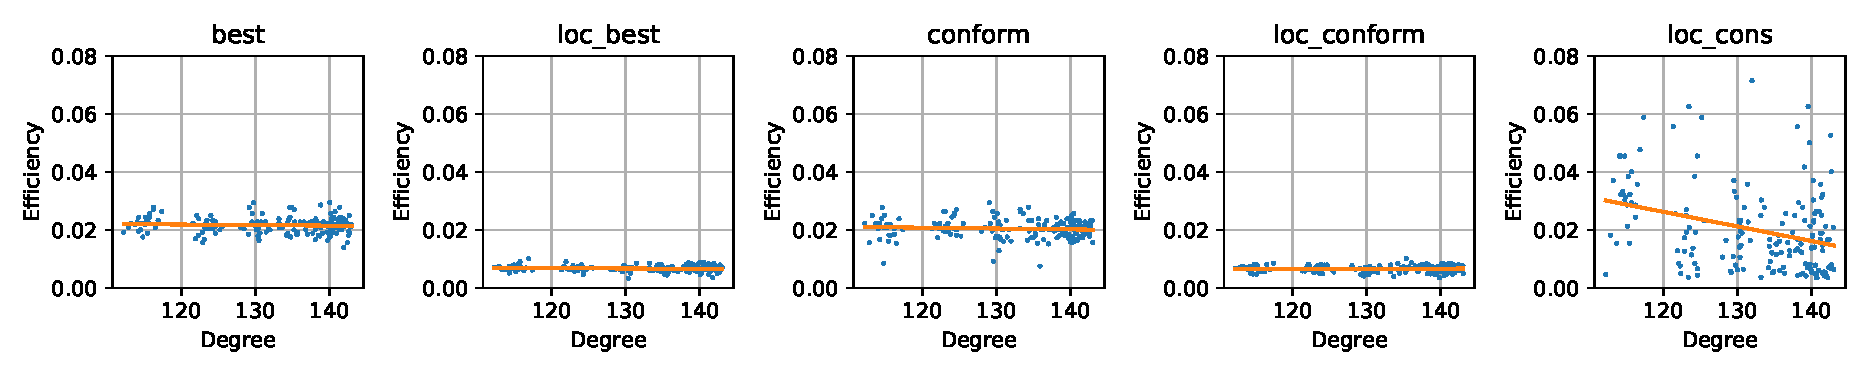
\includegraphics[width=6.67in,height=1.33in]{fig-deg-eff.pdf}
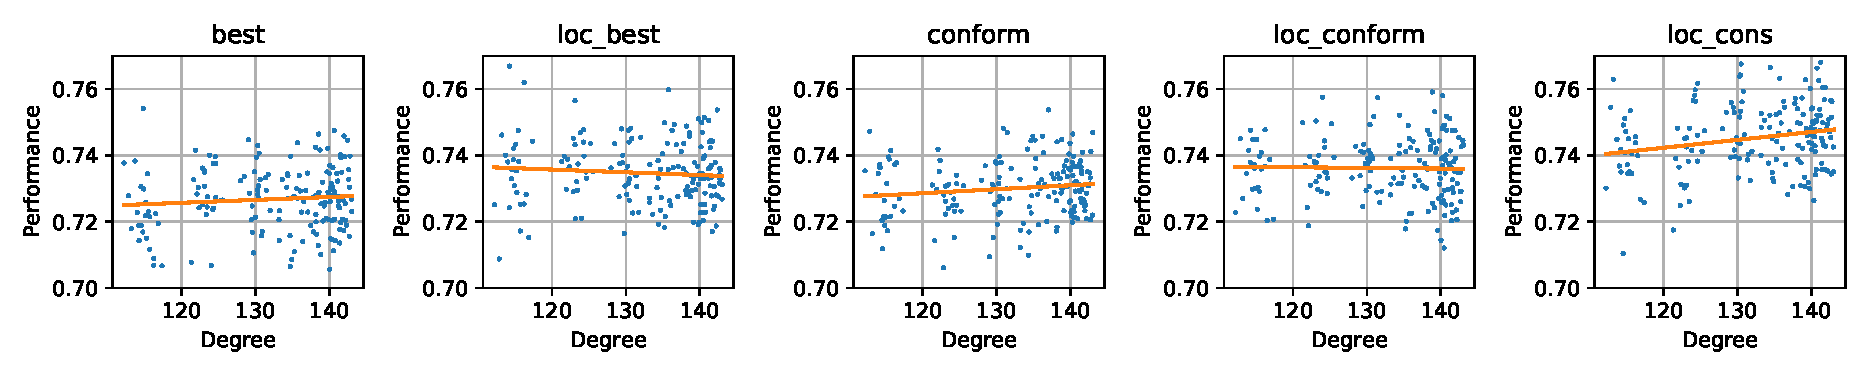
\includegraphics[width=6.67in,height=1.33in]{fig-deg-perf.pdf}
\caption{
Efficiency and Performance of social learning strategies vs network degree.
Each point represents a single trial of 300 iterations.
The consensus strategy shows increased performance and decreased efficiency as
degree increases, while other strategies show no degree dependence.
\label{fig:deg-eff-perf}
}
\end{figure*}

Figure \ref{fig:val-iter} shows how agents' solutions improve after repeated applications of
different learning strategies and rewiring values.
Each curve represents an average over 100 trials, each with 250 agent solutions.
For all rewiring values, local strategies are less efficient and more performant than their
non-local counterparts.
The consensus strategy is both more efficient and more performant than others,
with its performance increasing with higher rewiring.

The effect of degree on performance and efficiency is shown in Figure \ref{fig:deg-eff-perf} and
Tables \ref{tab:sim-eff} and \ref{tab:sim-perf}.
For both local and non-local versions of the best-neighbor and conformity strategies,
there is no significant effect of degree on performance or efficiency.
As noted above however, the local versions consistently have higher performance and lower efficiency
than their non-local counterparts.
We observe more interesting behavior with the consensus strategy.
Node degree shows a significant negative correlation with degree,
and a small but significant positive correlation with efficiency.
The consensus simulations replicate the efficiency behavior observed in WikiProjects,
but the opposite behavior for performance.
But unlike other strategies, consensus demonstrates that degree distribution can have an
impact on both performance and efficiency.

\section{Discussion}
\label{sec:discuss}

While existing research into the role of network structure in collaboration
has focused on numerical simulations and lab experiments,
analysis of large real-world systems is an important next step.
Our empirical analysis of WikiProjects contributes several findings towards a better
understanding of large, decentralized, real-world collaboration.
We observe several results consistent with previous work:
a trade-off between performance and efficiency,
higher performance for shorter path lengths in a conformity setting,
and a reduction in performance with increased structural inequality.
By using real-world networks, we were also able to analyze network properties independently,
allowing us to show that while most existing work has focused on the importance of path length,
degree distribution may be just as, or more, important.
The association of low-degree with both high performance and high efficiency is compelling,
as it sidesteps the usual trade-off between performance and efficiency.
In low-degree networks, agents have more repeated interactions with smaller groups of collaborators,
possibly suggesting that small team sizes could be beneficial for large collaborations.
Similarly, the observation that performance is higher in projects with less structural inequality suggests that,
if the challenges of egalitarian organizing can be overcome,
decentralized collaborations may produce better outcomes than those with centralized, top-down structures.

Our numerical simulations offer a few additional insights.
Our proposed local variants of best-neighbor and conformity strategies out-performed
the standard variants while searching fewer alternatives.
The higher performance for less work is analogous to the performance increases that
have been seen for sampling fewer neighbors \cite{barkoczi_social_2016}.
However, our network is a special case in that its structure is related to the structure of
the NK model being optimized, which could increase the usefulness of local information.
Our proposed consensus strategy, intended to model Wikipedia more closely,
exhibits a degree-dependent performance and efficiency, unlike other strategies.
This dependence is also seen in our Wikipedia analysis, although performance's dependence has the opposite sign.
The consensus strategy is also interesting in that it is more efficient and higher performance than the other strategies.
The unique properties of the consensus strategy may be due to a major difference it has from the others:
rather than exploring through local hill-climbing,
the consensus strategy combines parts of existing solutions to create entirely new ones.

Our work has several limitations.
Our empirical analysis is purely correlative and cannot be used to draw
conclusions about the causal influence of network structure on collaboration.
However, the consistency of our results with other lab-based and numerical studies
suggests that the causal link is worth further study.
Similarly, our study focuses entirely on a single setting and while it is suggestive,
does not necessarily generalize,
and studies of other systems are necessary to corroborate our findings.

Our work raises several questions that could be the subject of future work.
Is the correlation between network structure, performance, and efficiency causal?
A time-dependent analysis of our data could offer insight.
Are similar relationships observed in other large-scale collaborations?
Does varying degree independently of path length influence performance and efficiency in a controlled
lab setting?

\section{Conclusion}
\label{sec:conclusion}

In this paper, we have described the relationship between the structural properties of WikiProject
coeditor networks and the performance and efficiency of those networks.
As in other studies, we see a trade-off between performance and efficiency,
but not an absolute trade-off.
Some properties, such as low degree, are associated with both higher performance and higher efficiency.
We also find that the correlations between path length and performance are consistent with a conformity-based
social learning strategy, but not a greedy best-neighbor strategy.
We also observe improved performance in more decentralized project, as has been seen in small-scale lab experiments.
While the performance and efficiency of most previously-studied social learning strategies depend more on path length than
degree,
we have proposed a novel consensus learning strategy that is more realistic, more efficient, and higher performance than
existing strategies.
While the efficiency and performance of existing strategies do not exhibit any degree-dependence, our consensus strategy
demonstrates that degree-dependence is possible.
While additional work is needed to determine causal relationships and how generalizable our results are,
we have shown evidence that several phenomena predicted by numerical and small-scale lab experiments are present in a large,
real-world network.
And, we have identified new behaviors not explained by existing models, suggesting the need for alternate models.
Our results suggest that the success of large-scale collaborations may be aided by greater decentralization,
consensus or conformity-based decision-making, and more tightly-knit collaborations between smaller teams.

\section{Acknowledgments}
Anonymized for blind review.
%I would like to thank Daniel M. Romero for valuable guidance and feedback;
%Ceren Budak and Scott E. Page for their time and feedback;
%Danielle Livneh and Karthik Ramanathan for help collecting the data sets;
%Yan Chen and Tanya Rosenblat for feedback on the methodology;
%and the attendees of the May 25, 2017 MIT Center for Civic Media lab meeting and
%the Berkman-Klein Center's Cooperation Working Group for helpful feedback on
%preliminary results.
%This research was funded by the University of Michigan School of Information.